\documentclass [a4paper]{article}
\usepackage{graphicx, amsmath}
\usepackage[a4paper, total={8.5in, 13in}, margin=1in]{geometry}
\bibliographystyle{plain}
\usepackage{listings}
\usepackage{xcolor}
\lstset{
    language=Python,
    basicstyle=\ttfamily\small,
    keywordstyle=\color{blue},
    commentstyle=\color{gray},
    stringstyle=\color{red},
    showstringspaces=false,
    frame=single,
    breaklines=true,
    numbers=left,
    numberstyle=\tiny\color{gray},
    tabsize=4,
}

\title{MAT 196 Laboratory Exercise No.2}
\author{Jeanne Marie B. Quiñanola}
\date{\today}

\begin{document}

\maketitle

\section{Introduction}
In difference equations, the changes in states of a system are modeled over discrete intervals. In most cases, the discrete intervals represent time intervals, and therefore the letter \(t\) is used to denote the time variable.
A form of the difference equation that will be encountered most often is 
\[
x_{t + k} + a_1 x_{t+k-1} + \ldots + a_{k-1} x_{t+1} + a_k x_t = b_t, \quad t = 0, 1,\ldots\]

The order of the difference equation is \(k\), provided \(a_k \neq 0\). The coefficients are assumed to be real and the functions are real-valued. The coefficients \(a_j\), \(j = 1, \ldots, k\), can be functions of \(t\) and state variables \(x_i\) for \(i = t, \ldots, t + k - 1\). The function \(b_t\) on the right-hand side of the equation may depend on \(t\) but not on the state variables.

If the coefficients \(a_j\), \(j = 1, \ldots, k\) in the equation are constant or depend on \(t\) but do not depend on the state variables, then the difference equation is said to be linear. Otherwise, it is said to be nonlinear. In addition, if the difference equation is linear and \(b_t = 0\) for all \(t\), then it is said to be homogeneous; otherwise, it is said to be nonhomogeneous.

The method for finding the general solution to the \(k\)-th order, nonhomogeneous, linear difference equation involves the following steps.

\begin{enumerate}
    \item[(a)] Find the general solution to the homogeneous difference equation (\(b_t = 0\)), a solution depending on \(k\) arbitrary constants and \(k\) linearly independent solutions. (Recall that the \(k\) solutions \(x^1, \ldots, x^k\) are linearly independent if \(\sum_{i=1}^{k} a_i x^i = 0\) implies \(a_i = 0\) for \(i = 1, \ldots, k\)). Denote the general solution as \(x_h\). Then 
    \[
    x_h = c_1 x^1 + \ldots + c_k x^k = \sum_{i = 1}^k c_ix^i,
    \]
    where \(c_1, \ldots, c_k\) are constants, and \(x^1, \ldots, x^k\) are \(k\) linearly independent solutions of the homogeneous equation. (Note: The notation \(x^i\) means the \(i\)-th solution and not \(x\) raised to the power \(i\).) Any linear combination of solutions to the linear homogeneous difference equation is also a solution. This property is known as the superposition principle. The key to finding the general solution is to identify the \(k\) linearly independent solutions.

    \item[(b)] Find a particular solution to the nonhomogeneous difference equation, a solution with no arbitrary constants. Denote this particular solution as \(x_p\).

    \item[(c)] The sum of the general solution \(x_h\) and the particular solution \(x_p\) gives the general solution to the nonhomogeneous linear difference equation:
    \[
    x_t = x_h + x_p 
    \]
    If initial conditions \(x_0, x_1, \ldots, x_{k-1}\) are prescribed, then the constants \(c_1, c_2, \ldots, c_k\) can be uniquely determined.
\cite{linda}
\end{enumerate}

By understanding these concepts, this study explores a specific difference equation, investigating  its long-term behavior and convergence through simulation and analysis.
\section{Analysis and Discussion}
Consider the second-order,nonhomogeneous,linear difference equation

\[
6x_t + 5x_{t-1} + x_{t-2} = \left(\frac{1}{5}\right)^t
\]
for \( t > 2 \) with initial conditions \( x_0 = 0 \) and \( x_1 = 1 \).
\subsection*{Solution}
To find two linearly independent solutions, \(x^1\) and \(x^2\), assume the solution has the  form \(x_t = \lambda^t\) where \(\lambda \neq 0\).\\
Solving for the general solution, we have:
\begin{align*}
6\lambda^t + 5\lambda^{t-1} + \lambda^{t-2} &= 0 \\
\lambda^{t-2}(6\lambda^2 + 5\lambda + 1) &= 0 \\
6\lambda^2 + 5\lambda + 1 &= 0 \\
(3\lambda + 1)(2\lambda + 1) &= 0 \\
\lambda_1 = -\frac{1}{3}, \quad \lambda_2 &= -\frac{1}{2}
\end{align*}
The general solution to the homogeneous equation is given by:
\begin{align*}
x_t^h &= c_1\lambda_1^t + c_2\lambda_2^t  \\
x_t^h &= c_1 \left(-\frac{1}{3}\right)^t + c_2 \left( -\frac{1}{2} \right)^t
\end{align*}
To solve for the particular solution, assume \(x_t^p = A\left(\frac{1}{5}\right)^t\), and substitute into the given difference equation.
\begin{align*}
6A \left(\frac{1}{5}\right)^t + 5A \left(\frac{1}{5}\right)^{t-1} + A\left(\frac{1}{5}\right)^{t-2} &= \left(\frac{1}{5}\right)^t \\
6A + 25A + 25A &= 1 \\
56A &= 1 \\
A &= \frac{1}{56} \\
\end{align*}

Thus, the particular solution is:

\[
x_t^p = \frac{1}{56} \left(\frac{1}{5}\right)^t
\]

Hence,

\begin{align*}
x_t &= x_t^h + x_t^p \\
x_t &= c_1 \left(-\frac{1}{3}\right)^t + c_2 \left( -\frac{1}{2} \right)^t + \frac{1}{56} \left(\frac{1}{5}\right)^t.
\end{align*}
\newpage
To solve for the solution of \(x_t\) satisfying the initial conditions \(x_0 = 0\) and \(x_1 = 1\), we have:

\begin{align*}
&x_0 = c_1 \left(-\frac{1}{3}\right)^0 + c_2 \left( -\frac{1}{2} \right)^0 + \frac{1}{56} \left(\frac{1}{5}\right)^0 = 0 \\
&c_1 + c_2 + \frac{1}{56} = 0 \\
&c_1 + c_2 = -\frac{1}{56}
\end{align*}
\begin{align*}
&x_1 = c_1 \left(-\frac{1}{3}\right) + c_2 \left( -\frac{1}{2} \right) + \frac{1}{56} \left(\frac{1}{5}\right) = 1 \\
&-\frac{1}{3}c_1 -\frac{1}{2}c_2 + \frac{1}{280} = 1 \\
&-\frac{1}{3}c_1 -\frac{1}{2}c_2 = \frac{279}{280}
\end{align*}

Hence, we have the following system of equations.

\[
\begin{cases}
  c_1 + c_2 = -\frac{1}{56} \\
  -\frac{1}{3}c_1 -\frac{1}{2}c_2 = \frac{279}{280}
\end{cases}
\]

Solving for \(c_1\) and \(c_2\), we have:

\begin{align*}
-\frac{1}{3}c_1 -\frac{1}{2}\left(-\frac{1}{56} -c_1\right) &= \frac{279}{280} \\
-\frac{1}{3}c_1 + \frac{1}{112} + \frac{1}{2}c_1 &= \frac{279}{280} \\
\frac{-2c_1 + 3c_1}{6} &= \frac{279}{280} - \frac{1}{112} \\
c_1 &= \left(\frac{79}{80}\right)(6) \\
c_1 &= \frac{237}{40}\\
c_2 &= -\frac{1}{56} - \frac{237}{40}\\
c_2 &= -\frac{208}{35}
\end{align*}

Thus,
\[
x_t = \frac{237}{40}\left(-\frac{1}{3}\right)^t -\frac{208}{35}\left(-\frac{1}{2}\right)^t + \frac{1}{56}\left(\frac{1}{5}\right)^t.
\]

\subsection{Convergence Analysis}
In order to determine the convergence of divergence of \(x_t\) we have the following. 
\begin{align*}
\lim_{t \to \infty} x_t &= \lim_{t \to \infty}\left[\frac{237}{40}\left(-\frac{1}{3}\right)^t - \frac{208}{35}\left(-\frac{1}{2}\right)^t + \frac{1}{56}\left(\frac{1}{5}\right)^t\right] \\
&= \frac{237}{40}\lim_{t \to \infty}(-1)^t \left(\frac{1}{3}\right)^t -\frac{208}{35}\lim_{t \to \infty} (-1)^t\left(\frac{1}{2}\right)^t + \frac{1}{56}\lim_{t \to \infty}\left(\frac{1}{5}\right)^t\\
&= \frac{237}{40} (0) - \frac{208}{35} (0) + \frac{1}{56} (0)\\
&= 0
\end{align*}

Thus, \(x_t\) converges to 0 as \(t \to \infty\).
\newpage
\section{Numerical Simulations}
The following is the graph of  the solution of \(6x_t + 5x_{t-1} + x_{t-2} = \left(\frac{1}{5}\right)^t\) with the given initial conditions \(x_0 = 0\) and \(x_1 = 1\).
\begin{figure}[h]
    \centering
    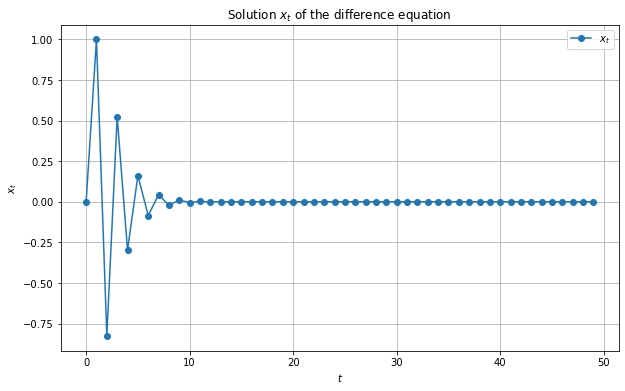
\includegraphics[width=1\textwidth]{MAT 196 Lab Activity 2}
\end{figure}

\noindent Here is the Python code for solving and plotting the difference equation:

\begin{lstlisting}
import numpy as np
import matplotlib.pyplot as plt

# Parameters of the equation
a = 6  # coefficient of x_t
b = 5  # coefficient of x_{t-1}
c = 1  # coefficient of x_{t-2}
initial_conditions = [0, 1]  # x_0 = 0, x_1 = 1
T = 50  # number of time steps to simulate

# Initialize the array to store the solution
x = np.zeros(T)
x[0], x[1] = initial_conditions

# Solve the difference equation iteratively
for t in range(2, T):
    x[t] = ((1/5)**t - b * x[t-1] - c * x[t-2]) / a
# Plotting the results
plt.figure(figsize=(10, 6))
plt.plot(np.arange(T), x, label=r'$x_t$', marker='o')
plt.title(r'Solution $x_t$ of the difference equation')
plt.xlabel(r'$t$')
plt.ylabel(r'$x_t$')
plt.grid(True)
plt.legend()
plt.show()
\end{lstlisting}

\section{Summary and Conclusions}
In this study, we examined the solution of a difference equation represented by \(x_t\). We derived both the homogeneous and particular solutions, ultimately combining them to formulate the general solution. We then implemented a Python code to simulate the behavior of \(x_t\) over time, utilizing specific parameters and initial conditions. The results were plotted to visualize the progression of \(x_t\) across a defined number of time steps.

The analysis and computational simulation indicate that as \(t\) approaches infinity, the values of \(x_t\) converge towards zero. This conclusion is visually supported by the graph generated through the Python code, which illustrates the diminishing behavior of \(x_t\) over time. Thus, our findings confirm that indeed, \(x_t\) converges to \(0\), reinforcing the theoretical predictions made throughout this study. This convergence is essential for understanding the long-term behavior of the system described by the difference equation.
\bibliography{citation} 
\end{document}
 